%\begin{tcolorbox}
%Teilt eure Klassendiagramme bitte auf und baut \textbf{kein} einzelnes riesiges Diagramm.
%Getter und Setter Methoden müssen hier nicht modelliert werden.
%Sie sollten aber der klassischen Namenskonvention folgen, um die Nutzung in Sequenzdiagrammen zu ermöglichen.
%\\\\
%Auf jedes Diagramm folgt eine Tabelle, in der die Aufgabe \textbf{jeder} Klasse beschrieben wird.
%\end{tcolorbox}

\section{Frontend}

\subsection{Web}

\begin{figure}[h]
	\centering
	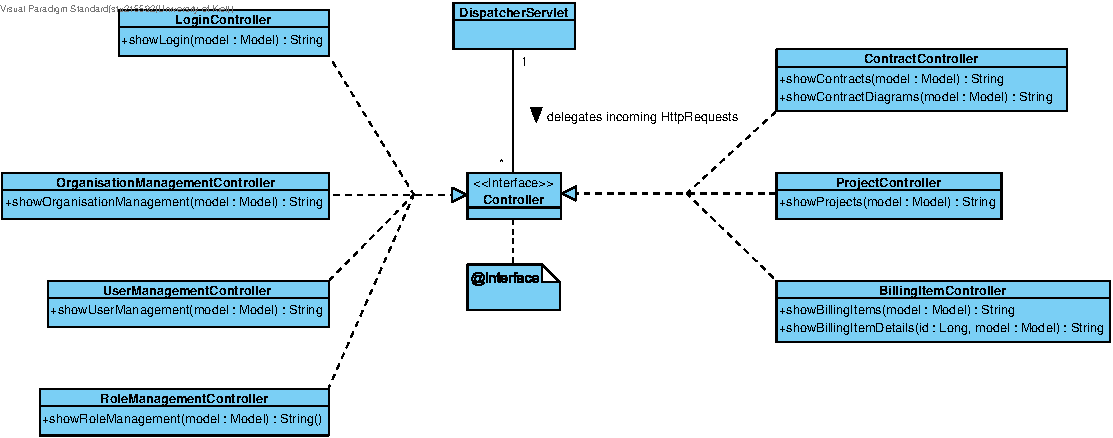
\includegraphics[width=\linewidth]{img/diagrams/Frontend Classes.pdf}
	\caption{Klassendiagramm - Frontend Web}
	\label{fig:klassendiagramm-web}
\end{figure}

\noindent
Klassen, deren Name mit ''Controller'' aufhört, verarbeiten HTTP Requests zu bestimmten Pfaden.
Die zu verarbeitenden Pfade sind pro Gebiet in einem jeweiligen Controller gruppiert.
In der folgenden Tabelle werden für Controller unter ''Aufgabe'' die zu verarbeitenden Pfade sowie die Bedeutung der dazugehörigen Seite aufgeführt.
Die Identifikationsnummern oID (Organisation), diaID (Diagramm), pID (Projekt), cID (Vertrag) und bID (Leistungsposition) sind in manche Pfade direkt integriert. \\

\centering
\begin{longtable}[h]{p{5.3cm} p{8.7cm}}
	\caption{Klassenbeschreibung - Frontend Web}
	\label{table:klassenbeschreibung-web}
	\endlastfoot
	\multicolumn{2}{r}{{Weitergeführt auf der folgenden Seite}} \\
	\endfoot
	\endhead
	\rowcolor[HTML]{C0C0C0} 
	\textbf{Klassenname} & \textbf{Aufgabe} \\
    
	DispatcherServlet & Teil des Spring Frameworks, leitet die HTTP Requests an den jeweils zuständigen Controller weiter \\
	
	\rowcolor[HTML]{E7E7E7} 
	LoginController & /login $\rightarrow$ Login-Seite \\
	
	OrganisationManagementController & /organisation\_overview $\rightarrow$ Management von Organisationen und deren OrgAdmins \\
	
	\rowcolor[HTML]{E7E7E7} 
	UserManagementController & /user\_overview $\rightarrow$ Management aller WebUser \newline\newline
	/organisation/\{oID\}/user\_overview $\rightarrow$ Management der WebUser einer Organisation \newline\newline
	/organisation/\{oID\}/add\_user $\rightarrow$ Hinzufügen eines WebUsers zu einer Organisation \newline\newline
	/role\_overview $\rightarrow$ Management aller Rollen \newline
	/organisation/\{oID\}/role\_overview $\rightarrow$ Management der Rollen einer Organisation \newline\newline
	/organisation/\{oID\}/add\_role $\rightarrow$ Hinzufügen einer Rolle zu einer Organisation \\
	
	ProjectController & /project\_overview $\rightarrow$ Zeigt alle Projekte an, für welche der WebUser die nötigen Berechtigungen hat \newline\newline
	/project/\{pID\}/show $\rightarrow$ Zeigt die Verträge des Projekts an, für welche der WebUser die nötigen Berechtigungen hat \\
	
	\rowcolor[HTML]{E7E7E7} 
	ContractController & /contract\_overview $\rightarrow$ Zeigt alle Verträge an, für welche der WebUser die nötigen Berechtigungen hat \newline\newline
	/project/\{pID\}/contract/\{cID\}/show $\rightarrow$ Zeigt die Leistungspositionen des Vertrags an, für welche der WebUser die nötigen Berechtigungen hat \newline\newline
	/diagram\_overview $\rightarrow$ Zeigt alle Diagramme an, für welche der WebUser die nötigen Berechtigungen hat \newline\newline
	/project/\{pID\}/contract/\{cID\}/create\_diagram $\rightarrow$ Erstellen eines Diagramms \newline\newline
	/project/\{pID\}/contract/\{cID\}/diagram/\{diaID\}/show $\rightarrow$ Zeigt das Diagramm im Detail an \\
	
	BillingItemController & /billing\_item\_overwiew $\rightarrow$ Zeigt alle Leistungspositionen an, für welche der WebUser die nötigen Berechtigungen hat \newline\newline
	/project/\{pID\}/contract/\{cID\}/billing\_item/\{bID\}/show $\rightarrow$ Zeigt Details zur Leistungsposition an
\end{longtable}

\clearpage

\section{App}

\section{Backend}

\subsection{Datenmodell}

\subsection{Datenverarbeitung}

\begin{figure}[h]
	\centering
	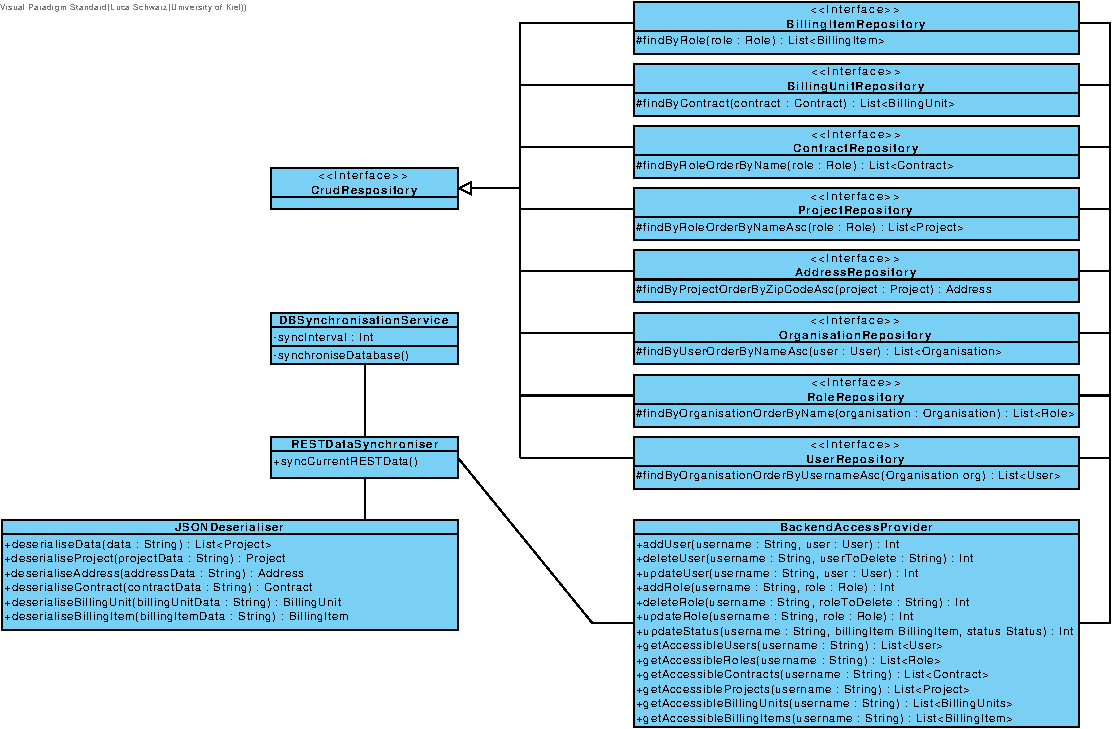
\includegraphics[width=\linewidth]{img/diagrams/Backend.pdf}
	\caption{Klassendiagramm - Backend - Datenverarbeitung}
	\label{fig:klassendiagramm-backend-data}
\end{figure}

\centering
\begin{longtable}[h]{p{5cm} p{9cm}}
	\caption{Klassenbeschreibung - Backend - Datenverarbeitung}
	\label{table:klassenbeschreibung-backend-data}
	\endlastfoot
	\multicolumn{2}{r}{{Weitergeführt auf der folgenden Seite}} \\
	\endfoot
	\endhead
	\rowcolor[HTML]{C0C0C0} 
	\textbf{Klassenname} & \textbf{Aufgabe} \\
	CrudRepository & Teil des Spring Frameworks. Wird hier genutzt, um die Datenbank in From von erbenden Repositories darzustellen \\
	\rowcolor[HTML]{E7E7E7} 
	*Repository & Verwaltet die jeweilige Datenmodellklasse. Bietet spezielle Zugriffsfunktionen für eine einfachere Nutzung \\
	BackendAccessProvider & Bietet die eigentliche Funktionalität des Backends innerhalb der Server-Applikation an. Über diese Klasse wird der gesicherte Zugriff auf die gespeicherten Daten sichergestellt und die 
    einzelnen DatenRepositories werden vor dem Nutzer verborgen. Alle Methoden verlangen einen Nutzernamen als Parameter, um festzustellen welche Daten tatsächlch zurückgegeben werden dürfen. Dafür werden intern die Rollen verwendet.
    So soll ein Nutzer z.Bsp. nur Zugriff auf Verträge bekommen für welche er über eine entsprechende Rolle verfügt. Ansonsten werden leere Listen und auch Fehlercode zurückgegeben, welche dann z.Bsp. vom Frontend
    entsprechen verarbeitet werden können. \\
	\rowcolor[HTML]{E7E7E7} 
	DBSynchronisationService & Dienst, welcher die Aufgabe hat nach einer gewissen verschrittenen Zeit eine Synchronisation der Datenbeank mit der von adesso zu veranlassen. Die Eigentliche Synchronisation wird
    durch die Klasse RESTDataSynchroniser durchgeführt. \\
    RESTDataSynchroniser & Hat zur Aufgabe die Daten über die REST-API von adesso abzufragen und folgend die Daten zu deserialisieren. Die so erhaltenen Klassen werden abschließend in die Datenbank eingeplegt. \\
	\rowcolor[HTML]{E7E7E7} 
	DBToJSONSerialiser & Dient dazu den gesamten Inhalt der Datenbank zu einen JSON-String zu konvertieren. Die ist notwendig um die App mit allen Daten zu versorgen auf die der AppUser Zugriff haben darf. \\
    JSONDeserialiser & Deserialisiert JSON-Strings zu den entsprechenden Modellklassen. Dies wird dann genutzt, wenn die über die REST-API von adesso Daten abgefragt werden. \\
    \rowcolor[HTML]{E7E7E7}
    JSONSerialiser & Serialisiert alle Modelklassen zu entsprechenden JSON-Strings. Diese Funktionalität wird vom DBToJSONSerialiser genutzt. \\
\end{longtable}